\documentclass[twoside, 12pt]{article}

\usepackage[sc]{mathpazo} % Use the Palatino font
\usepackage[T1]{fontenc} % Use 8-bit encoding that has 256 glyphs
\linespread{1.5} % Line spacing - Palatino needs more space between lines

%\usepackage[twoside,width=16cm,height=24cm,left=3cm]{geometry}
\usepackage[hmarginratio=1:1,top=20mm,width=20cm,height=23.7cm,columnsep=15pt]{geometry} % Document margins
\usepackage{multicol} % Used for the two-column layout of the document
\usepackage[hang, small,labelfont=bf,up,textfont=it,up]{caption} % Custom captions under/above floats in tables or figures
\usepackage{booktabs} % Horizontal rules in tables
\usepackage{float} % Required for tables and figures in the multi-column environment - they need to be placed in specific locations with the [H] (e.g. \begin{table}[H])
\usepackage{hyperref} % For hyperlinks in the PDF

%----------- Agregados para el caso de ustedes -------------------------------
\usepackage[spanish]{babel}% idioma castellano
\usepackage[utf8]{inputenc}% esto es para poder poner los tildes directamente.
\usepackage{graphicx} % para insertar figuras
\usepackage{subfigure} % para insertar figuras dentro de figuras
\usepackage{times} % plataforma
\usepackage{amsmath} % --para ecuaciones y algunos símbolos 
\usepackage{wrapfig,lipsum}
\usepackage{listings}
\usepackage{color}

\definecolor{dkgreen}{rgb}{0,0.6,0}
\definecolor{gray}{rgb}{0.5,0.5,0.5}
\definecolor{mauve}{rgb}{0.58,0,0.82}

\lstset{frame=tb,
	language=C++,
	aboveskip=3mm,
	belowskip=3mm,
	showstringspaces=false,
	columns=flexible,
	basicstyle={\small\ttfamily},
	numbers=none,
	numberstyle=\tiny\color{gray},
	keywordstyle=\color{blue},
	commentstyle=\color{dkgreen},
	stringstyle=\color{mauve},
	breaklines=true,
	breakatwhitespace=true,
	tabsize=3
}
% ---------------------- -----------------------------------------------------

\usepackage{lettrine} % The lettrine is the first enlarged letter at the beginning of the text
\usepackage{paralist} % Used for the compactitem environment which makes bullet points with less space between them
\usepackage[T1]{fontenc}					%para poder usar tildes sin problemas

\usepackage{mathrsfs}
% Abreviaturas
%\newcommand\RR{\mathbb{R}}

\graphicspath{{Imagenes/}}

\begin{document}
	
\begin{center}
	{\fontsize{20pt}{10pt}\textbf{Implementación de Morse en pexmd}}
\end{center}

Con el objetivo de probar la implementación del potencial de Morse, corrimos simulaciones para obtener la curva de E(T) y compararla con la obtenida en LAMMPS. 
Como el método de reescalamiento de velocidades no funcionaba para controlar la temperatura, debimos implementar un termostato de Andersen. 

\section{Morse Interaction Class}

Implementamos el potencial de Morse en \texttt{Python} como una clase heredada de \texttt{ShortRange}

\[ V_{M} (r) = D\left[1-e^{-\alpha (r-r_{eq})}\right]^2\]

Por lo tanto, la clase tiene métodos \texttt{pair\_force}, \texttt{pair\_energ} y \texttt{forces}, utilizando las implementación óptimas \texttt{forces9} en \texttt{C} discutida en \textbf{Compiladores}. 
En este aspecto, las funciones de \texttt{Python} no son más que wrappers (encapsulamiento) de sus contrapartes en \texttt{C}. Este aspecto es general para las interacciones de tipo \texttt{ShortRange}; 
lo mismo ocurre en la implementación de Lennard-Jones. 

La clase de \texttt{Python} está definida en \texttt{morse\.py} e importa una librería dinámica \texttt{morse\_pot.so} con las funciones de \texttt{morse\_pot.c}

\section{Prueba del potencial de Morse}

Tomamos parámetros arbitrarios para el potencial de Morse (con partículas de masa $m=1$)
\[ \left\{\begin{matrix}
D = 0.5 & \alpha = 1.0 \\
r_{eq} = 1.0 & r_{cut} = 2.5\\
\end{matrix} \right. \]

Buscamos reproducir la curva $E(T)$ para $1\leq T\leq 10$ a una densidad $\rho = 2$ ($N_{part}=512$, $L=6.3496$).

\subsection{Corrida en LAMMPS}

Dado que en \texttt{pexmd} no teniamos implementadas las condiciones de contorno periódicas, utilizamos inicialmente las \texttt{fixed}. 
Sin embargo, inmediatamente hubo problemas con partículas escapando de la caja. Esto no ocurría para las condiciones de contorno \texttt{periodic}, así que decidimos utilizarlas. 
Buscamos entonces que el sistema condense a una única una gota esférica, donde el $r_{cut}$ se encargaría que la gota no interactue con sus imagenes. 
En este régimen, las condiciones \texttt{fixed} y \texttt{periodic} deberían ser equivalentes. 
Se encontró para $\rho=2$ con $N_{part}=512$ y $L=6.3496$ y la gota puede apreciarse en la \textbf{Figura \ref{fig:gota}}.

\begin{figure}[h]
	\centering
	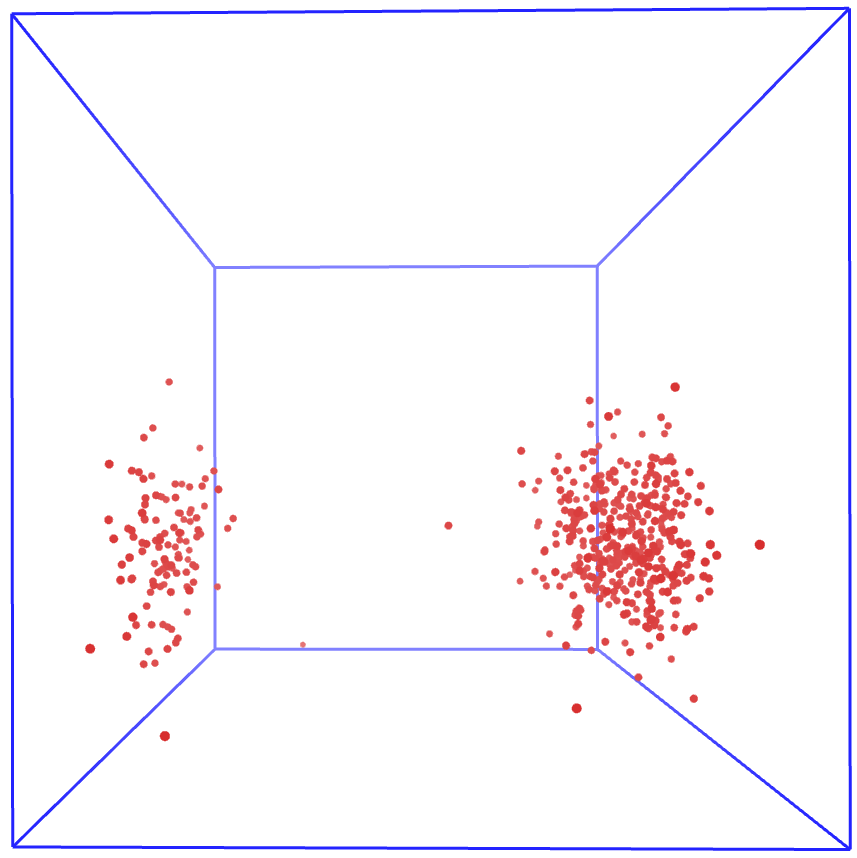
\includegraphics[width=0.5\columnwidth]{gota.png}
	\caption{Gota obtenida con \texttt{LAMMPS}, formada gracias a las condiciones de contorno periódicas.}
	\label{fig:gota}
\end{figure}

Usando el termostato de LAMMPS, registramos el par ($E$,$T$) en cada paso. La termalización comenzaba con un aumento hasta $T\sim 15$ donde se estancaba durante un largo tiempo previo a comenzar a bajar. Las pruebas 
preliminares con $\Delta t= 5\times 10^{-4}$ y $\Delta t= 5\times 10^{-3}$ no lograban alcanzar $T=10$ ni siquiera en $10^5$ pasos.

Por lo tanto, bajamos a $\Delta t = 0.05$ en una corrida de $1.5\times10^{5}$ pasos, donde la temperatura se comporta segun esperabamos (ver \textbf{Figura \ref{fig:temp_lammps}}). La corrida entera tomó $\sim 13$min y 
termalizó aproximadamente en el paso 120000. 
Analizando los valores de $T$ y $E$ a partir de ese paso, obtenemos la relación $E(T)$ de la \textbf{Figura \ref{fig:EvsT_lammps}}. Dado que el potencial Morse de \texttt{LAMMPS} difiere en una constante del implementado
en \texttt{PEXMD}, del ajuste lineal solo nos importa la pendiente, que en este caso resultó $m_{lammps}=1033$. Para confirmar la equivalencia, nos bastaría encontrar $m_{pexmd}\approx 1000$.

\begin{figure}[H]
	\centering
	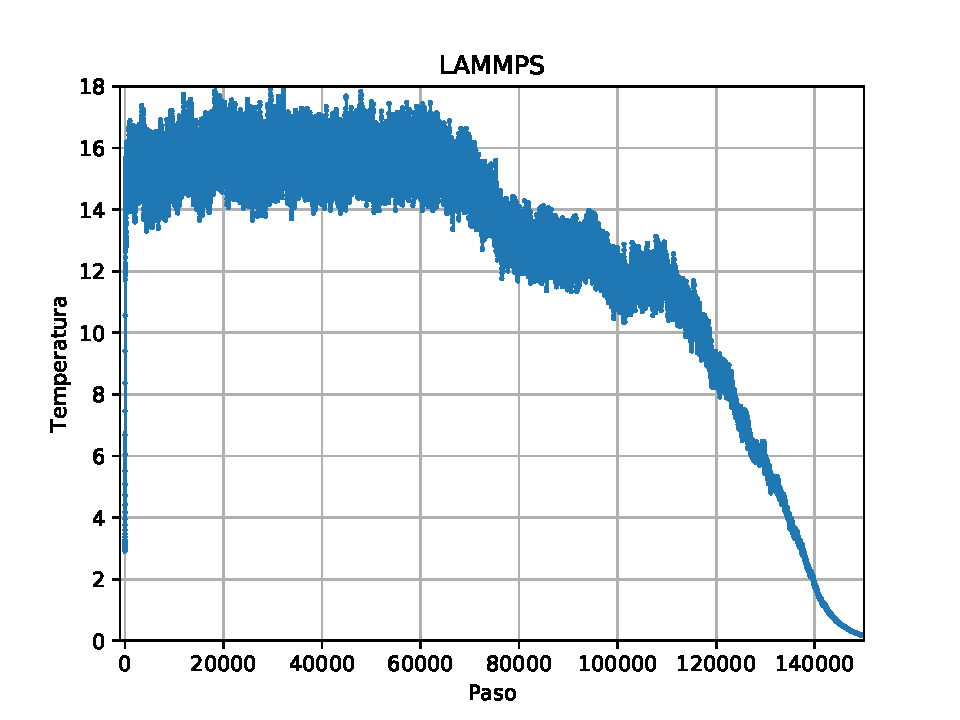
\includegraphics[width=0.5\columnwidth]{temp_lammps.pdf}
	\caption{Temperatura a lo largo de la simulación para $\Delta t = 0.05$ en LAMMPS (~13min). Termaliza aproximadamente a los 120000 pasos.}
	\label{fig:temp_lammps}
\end{figure}

\begin{figure}[H]
	\centering
	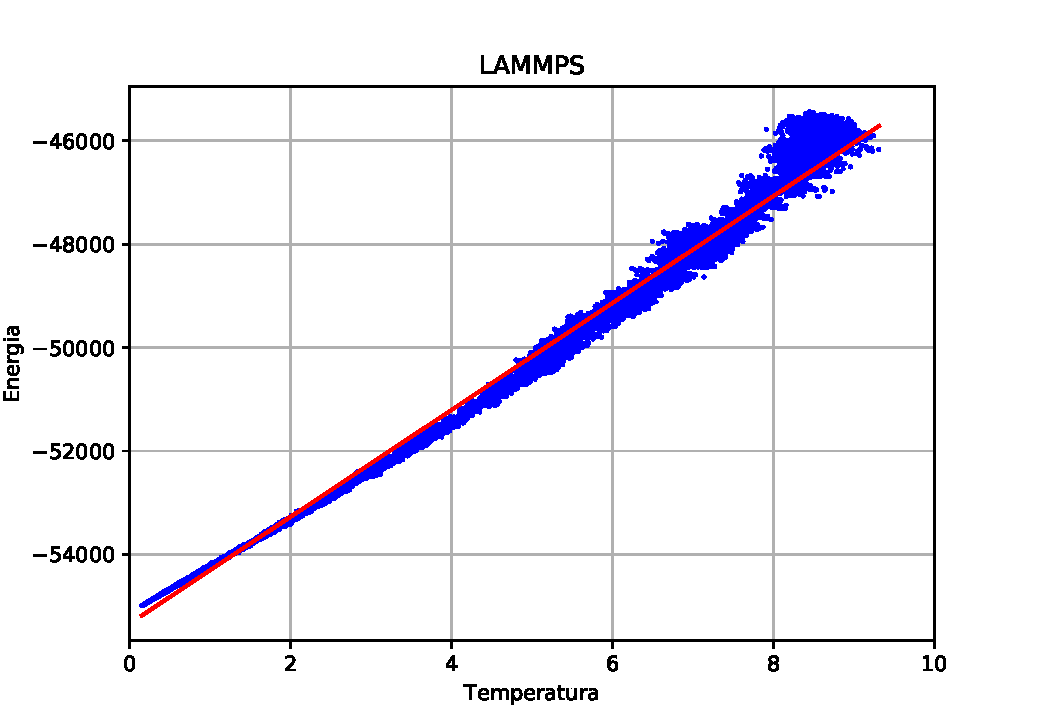
\includegraphics[width=0.5\columnwidth]{evt_lammps.pdf}
	\caption{Relación Energía-Temperatura obtenida con LAMMPS. El ajuste lineal arroja pendiente $m=1033$.}
	\label{fig:EvsT_lammps}
\end{figure}

% LAMMPS m = 1033
\subsection{Primeras corridas en PEXMD}

Pasando al código en \texttt{PEXMD} (\texttt{test\_morse.py}), primero buscamos el paso $\Delta t$ que aseguraba la conservación de la energía $E$. 
Probamos con $\Delta t = [4,3,2]\times10^{-2}$, obteniendo derivas considerables de energía al cabo de $100, 1000, 10000$ pasos, respectivamente. 
Recién para $\Delta t = 10^{-2}$ logramos que la energía se conserve para tiempos largos ($\sim 10^{5}$ pasos).

La primer corrida de $3\times10^{5}$ pasos tomó aproximadamente 80 minutos. 
Comparado con los 13 minutos que tomó la corrida de \texttt{LAMMPS} con la mitad de los pasos, estimamos que \texttt{PEXMD} tarda aproximadamente el triple. 
Esto puede deberse a que no implementamos una lista de primeros vecinos eficiente, sino que en la lista se encontraban todos los pares de partículas independientemente de su distancia.

El problema en todas estas corridas puede ser resumido analizando la última corrida con $5\times10^{5}$ pasos de la \textbf{Figura \ref{fig:sin_termo}}, donde puede verse que el método de reescalamiento de 
velocidades (cada 12500 pasos) utilizado para controlar la temperatura no resultó apropiado. Es claro que la temperatura sube incluso después de ser reescaladas las velocidades, impidiendo el muestreo. 
Además, las leves derivas en la energía sugerían un paso temporal más pequeño.

\begin{figure}[h]
	\centering
	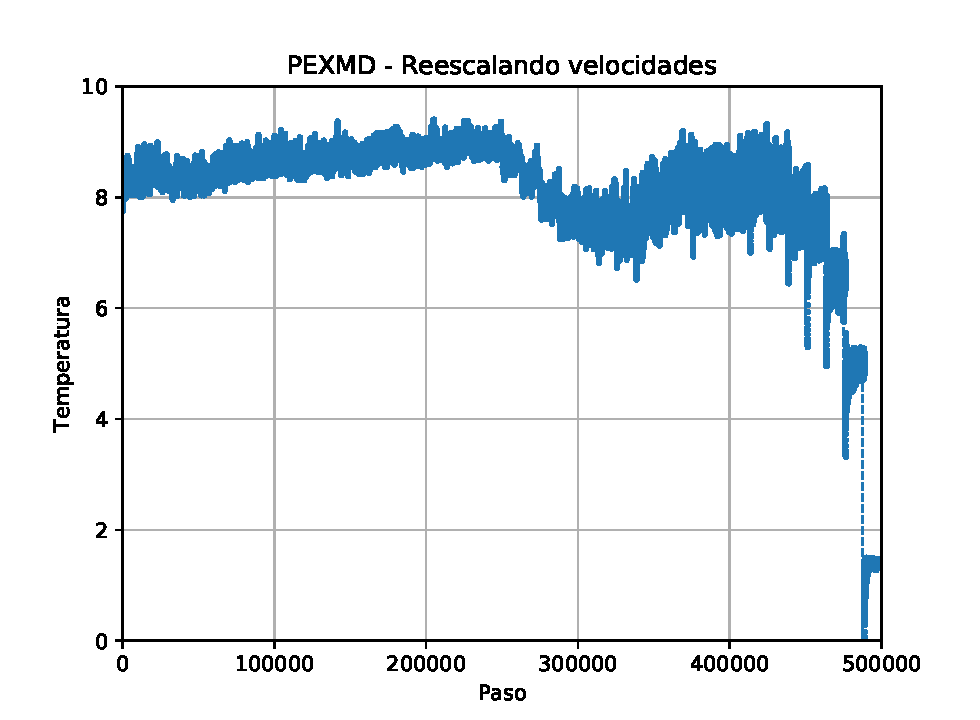
\includegraphics[width=0.47\columnwidth]{tsintermo_pexmd.pdf}
	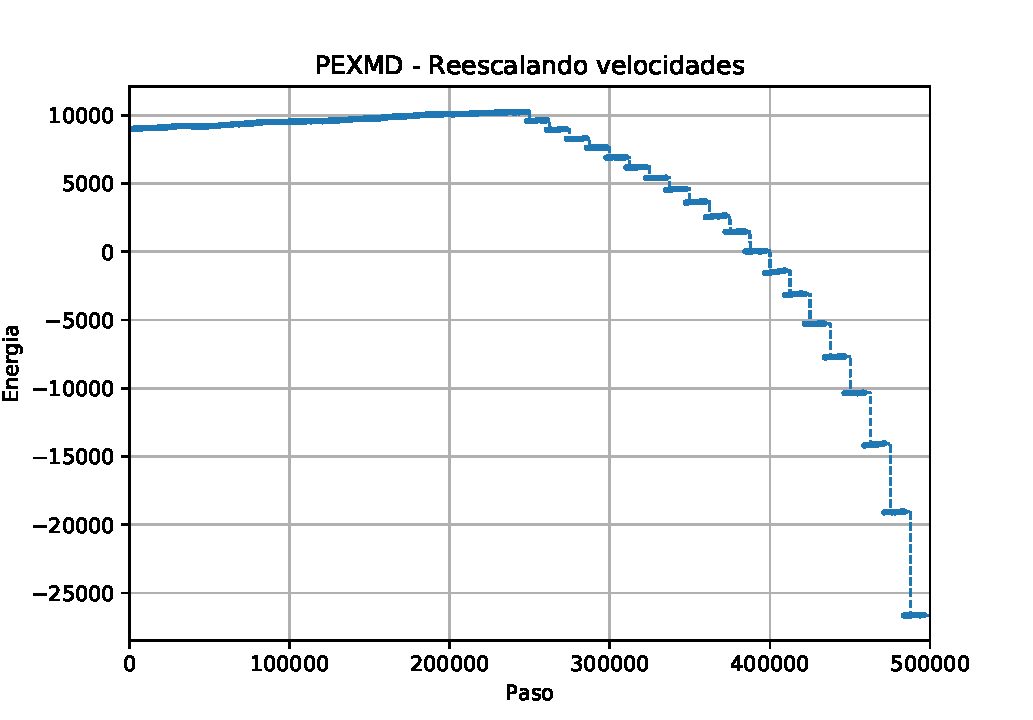
\includegraphics[width=0.49\columnwidth]{esintermo_pexmd.pdf}
	\caption{Energía y temperatura obtenidas para una corrida de 500000 pasos utilizando reescalamiento de velocidades para variar la temperatura. 
	Este método no es efectivo y solo parecería funcionar a temperaturas bajas}
	\label{fig:sin_termo}
\end{figure}

Creemos que la incapacidad del reescalamiento de velocidades de controlar la temperatura se debe a una distribución desigual de la energía total entre cinética y potencial.
Esto puede deberse a que el potencial de Morse no es de tipo \textit{hard-core} sino que en $r=0$ alcanza un máximo finito, lo cual acota su aporte energético.
En un choque, por lo tanto, la transmición de energía estaría acotado (de hecho, las partículas podrían atravesarse sin más).

\subsection{Termostato de Andersen y corridas finales en PEXMD}

Dada nuestra incapacidad de controlar la temperatura reescalando velocidades, decidimos implementar un simple termostato de Andersen.
Dado que este termostato puede utilizarse tanto para una integración NVE (Verlet, en nuestro caso) como NVT, resultó conveniente implementarlo como una clase aparte heredera de una clase \texttt{Thermostat} cuyo único
atributo fuese la temperatura $T$.

En particular, para Andersen debian también tomarse como parámetros la masa $Q$ y una semilla $seed$. 
Esto último se debe a que es un termostato estocástico, donde cada partícula tiene una probabilidad $Q$ de chocar, reiniciando su velocidad según la distribución de Boltzmann a esa dada $T$.
La semilla, por otro lado, se utilizó para inicializar una variable RandomState capaz de generar numeros aleatorios en base a esa semilla (reproducibilidad).

Entonces se probó utilizar este termostato, variando la temperatura entre 10 y 1 con el termostato. Las primeras pruebas mostraron que $Q=0.2$ resultaba excesivo, permitiendo la termalización en menos de 50 pasos. 
Esto es un problema, dado que valores de $Q$ altos pueden afectar las propiedades termodinamicas del sistema, dado que el $20\%$ del tiempo cada partícula tiene la velocidad que le correspondería a un gas igual.
Por lo tanto, tomamos $Q=0.05$, para lo cual la termalización tomaba aproximadamente 200 pasos, una cantidad de pasos razonable. 

Armados con este nuevo termostato, realizamos una corrida de $10^5$ pasos con temperatura inicial $T=10$ y bajando de $0.5$ hasta alcanzar $T=1$. 
La temperatura a lo largo de la evolución puede apreciarse en la \textbf{Figura \ref{fig:term_pexmd}}. 

\begin{figure}[h]
	\centering
	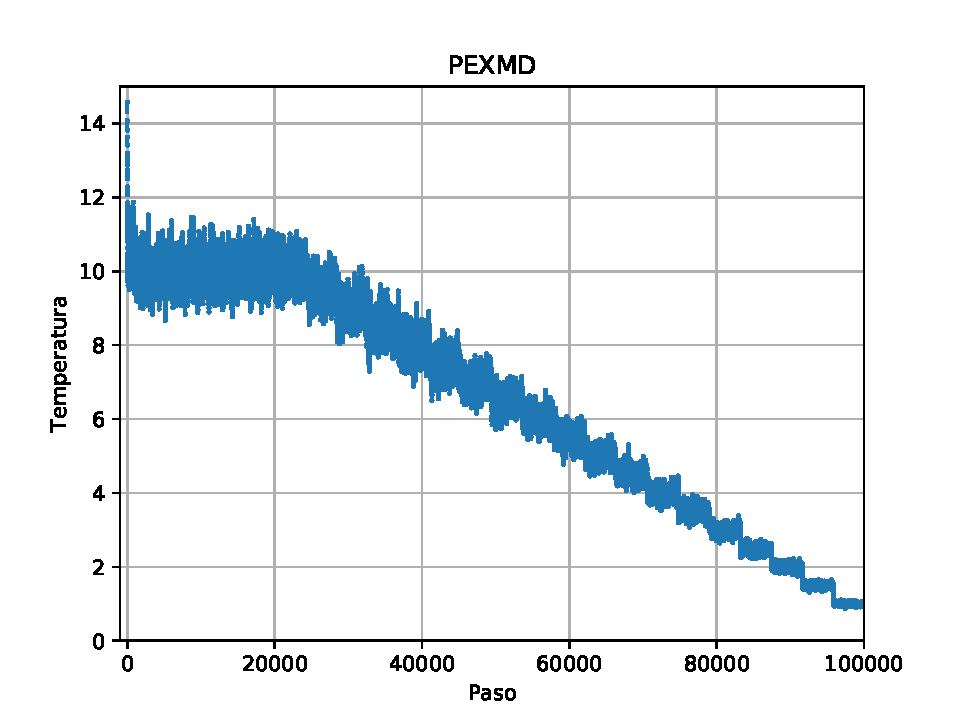
\includegraphics[width=0.5\columnwidth]{temp_pexmd.pdf}
	\caption{Temperatura a lo largo de la simulación. Los saltos corresponden pasos de $0.5$ de la temperatura $T$.}
	\label{fig:temp_pexmd}
\end{figure}

A partir de ahora, distinguiremos entre la temperatura del termostato $T$ y la temperatura medida $T_m = 2E_{cin}/3N_{part}$. 
Para analizar la calidad del termostato, podemos realizar un histograma de $T_m$ y $E$ para cada valor de $T$. Esperamos que el valor medio de $T_m$ coincida con $T$ según el teorema del virial 
y que el desvío estandar resulte pequeño.
Para evitar que interfieran lastermalizaciones intermedias, ignoramos los primeros 1000 pasos de cada $T$ y construimos los histogramas de la \textbf{Figura \ref{fig:histogramas}}. 
En ambos histogramas, tenemos una distribución unimodal según lo esperado. Es interesante notar que para $T_m$ se tiene $\mu\approx T$ y $\sigma/\mu \approx 0.035$ para las distintas $T$ (esto también se 
mantiene en las temperaturas no mostradas), por lo que las fluctuaciones relativas son constantes y pequeñas. 

\begin{figure}[h]
	\centering
	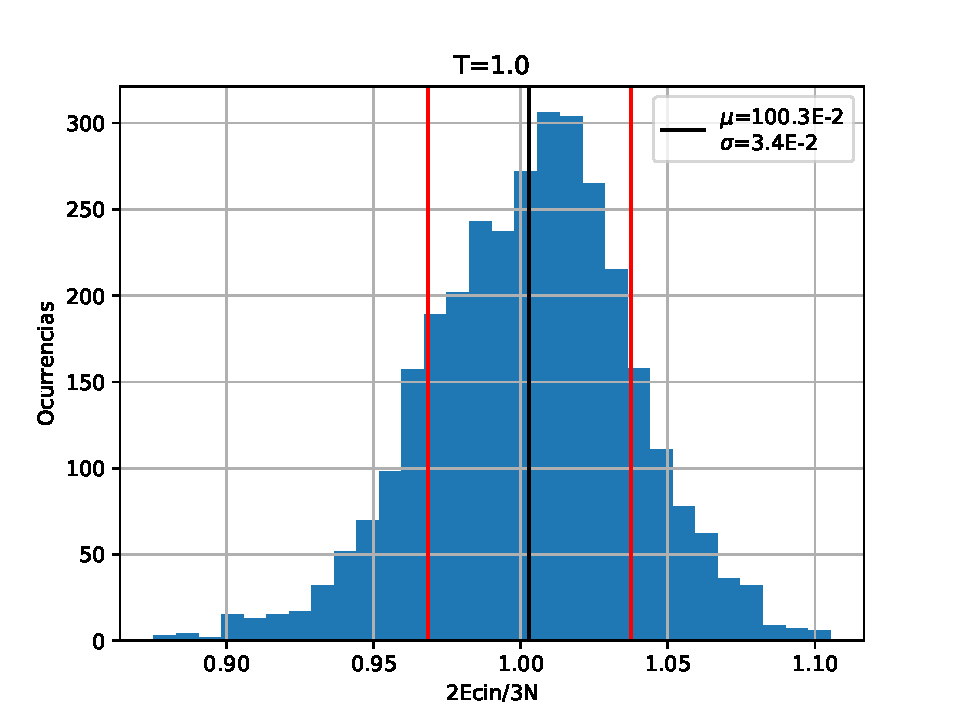
\includegraphics[width=0.32\columnwidth]{t_hist_1.pdf}
	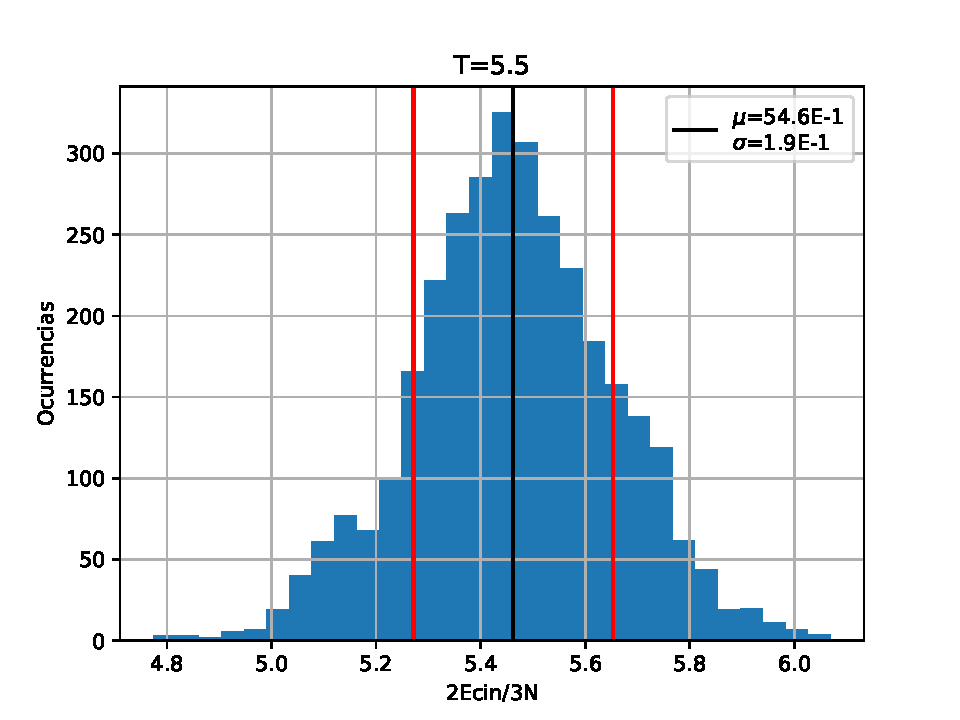
\includegraphics[width=0.32\columnwidth]{t_hist_5,5.pdf}
	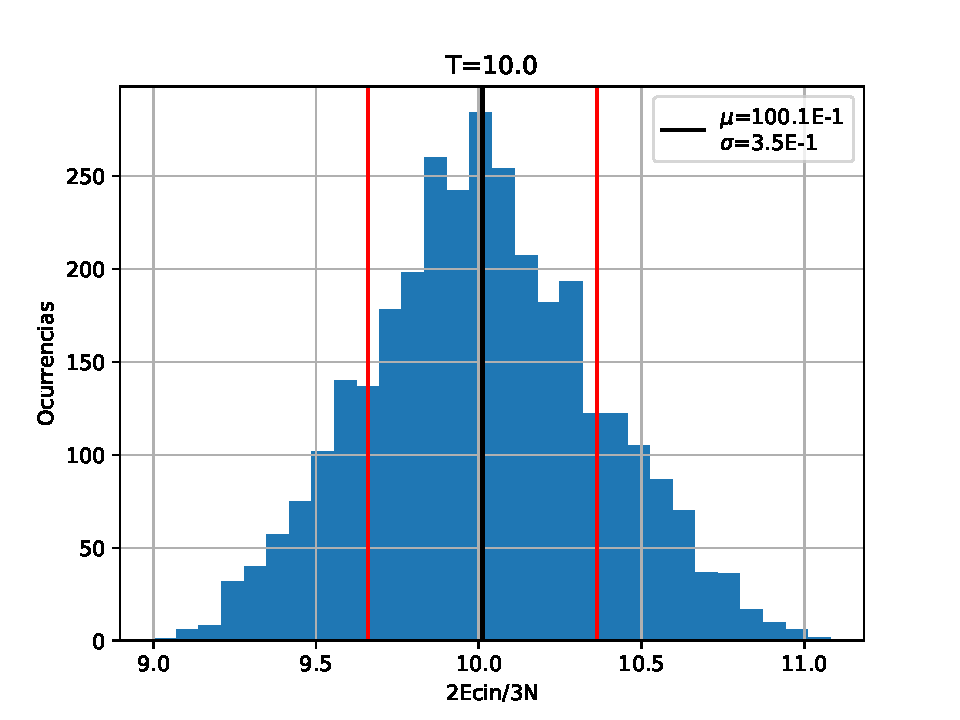
\includegraphics[width=0.32\columnwidth]{t_hist_10.pdf}
	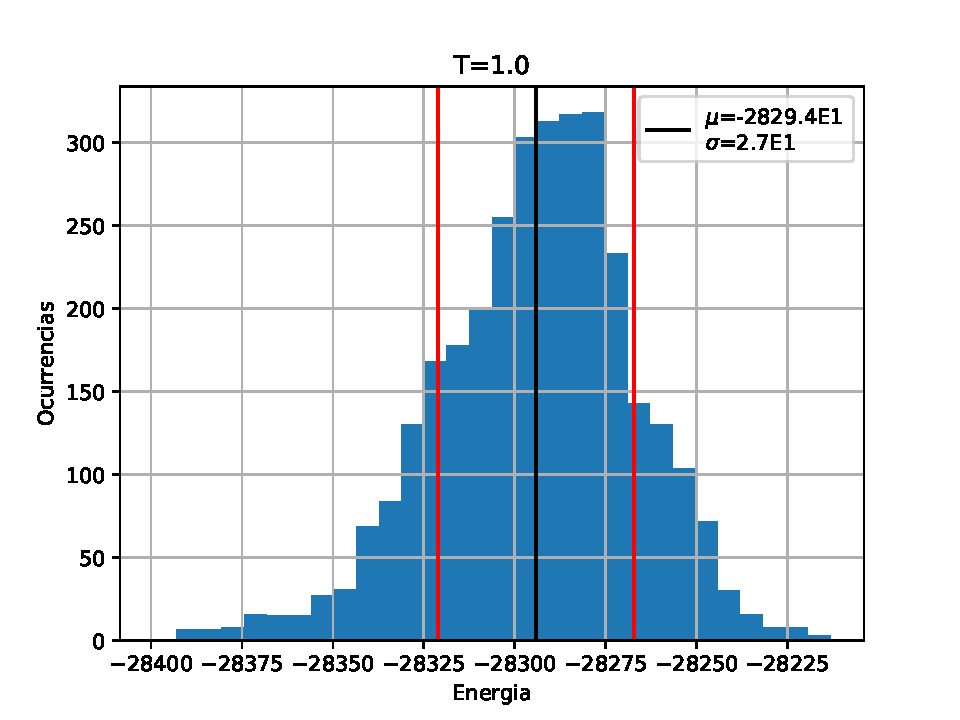
\includegraphics[width=0.32\columnwidth]{e_hist_1.pdf}
	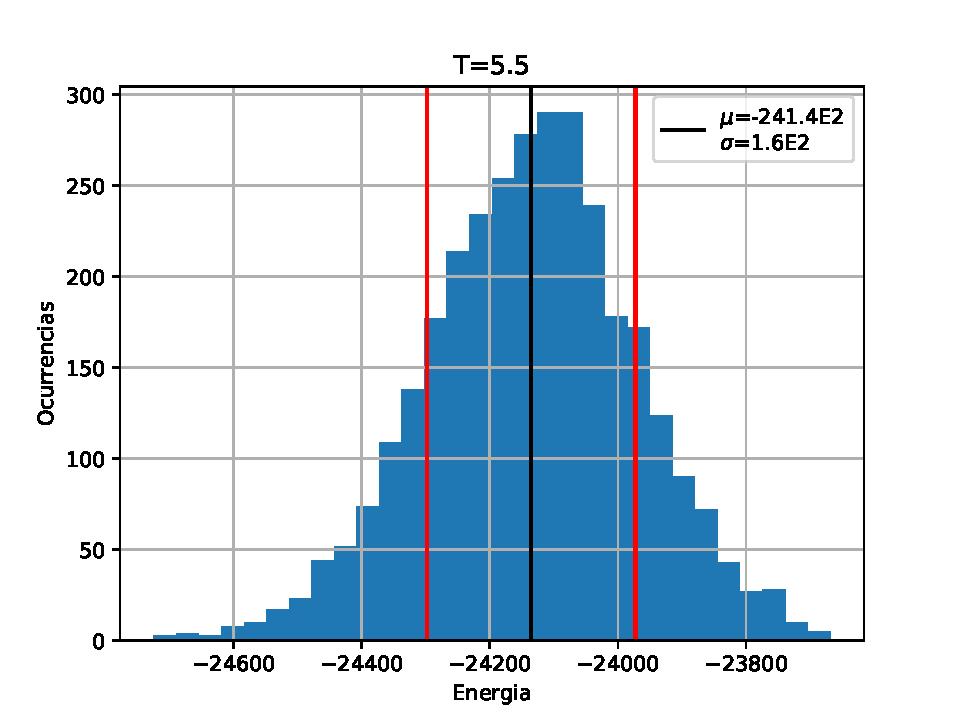
\includegraphics[width=0.32\columnwidth]{e_hist_5,5.pdf}
	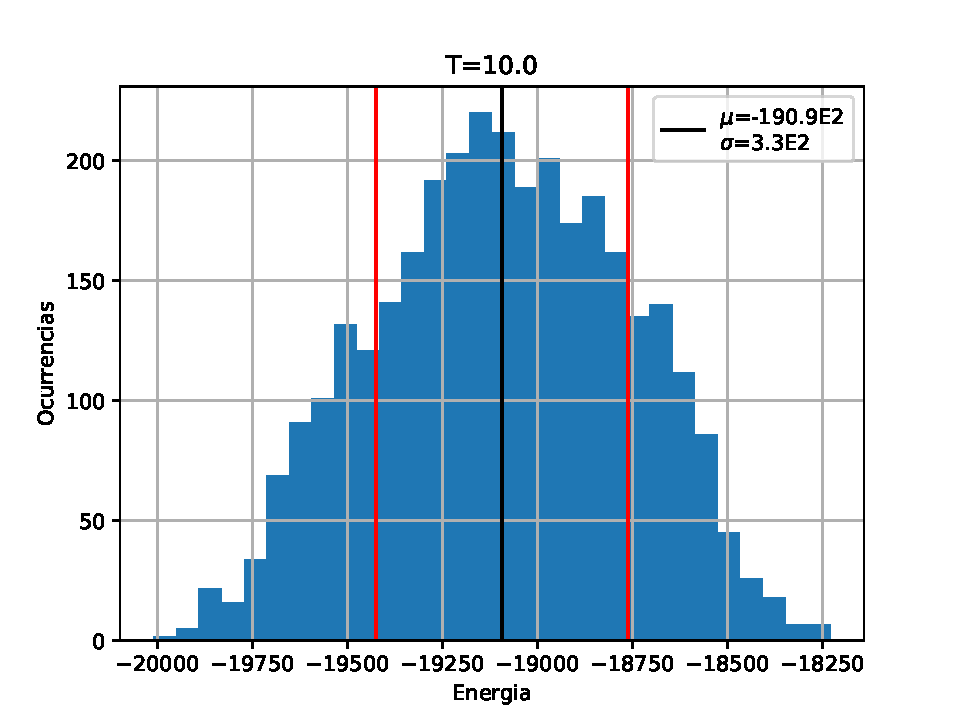
\includegraphics[width=0.32\columnwidth]{e_hist_10.pdf}
	\caption{Histogramas de $E$ y $T_m$ para 3 temperaturas características: alta, media y baja. Son unimodales y tienen un $T_m$ con $\mu\approx T$ y $\sigma/\mu \approx 0.035$ según lo esperado.}
	\label{fig:histogramas}
\end{figure}

En particular, graficamos $T_m$ en función de $T$ para confirmar el comportamiento lineal de pendiente 1 y ordenada nula. 
En la \textbf{Figura \ref{fig:EcinvsT}} podemos apreciar el ajuste lineal que arrojó pendiente $m=1.00288$ y ordenada $b=-0.0093$, coincidente con lo esperado.

\begin{figure}[H]
	\centering
	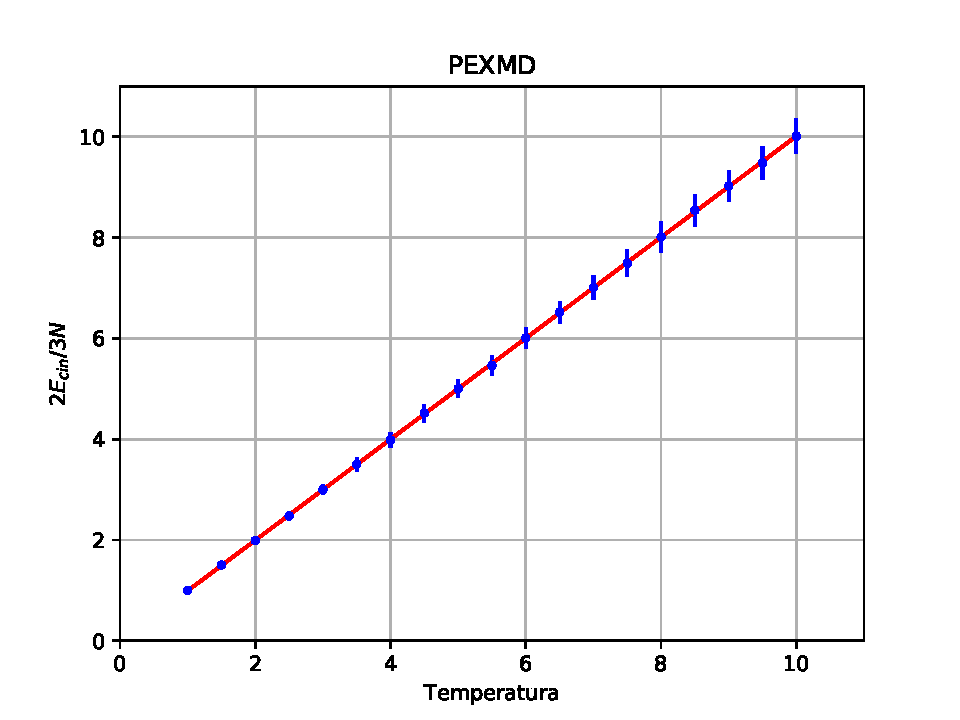
\includegraphics[width=0.5\columnwidth]{ecinvt_pexmd.pdf}
	\caption{Relación entre $T$ y la energía cinética. La pendiente $m=1.00288$ y ordenada $b=-0.0093$ del ajuste confirman la calidad del termostato.}
	\label{fig:EcinvsT}
\end{figure}

Finalizado este análisis, pasamos a graficar $E$ vs $T$ para confirmar que es consistente con lo obtenido para \texttt{LAMMPS}. 
Lo hacemos tanto con $T_m$ como con $T$, pero los resultados resultan muy similares y consistentes con lo anterior, con pendientes $m_{pexmd,1}=1011$ y $m_{pexmd,2}=1021$, respectivamente, muy similares 
a la anterior $m_{lammps}=1033$

\begin{figure}[H]
	\centering
	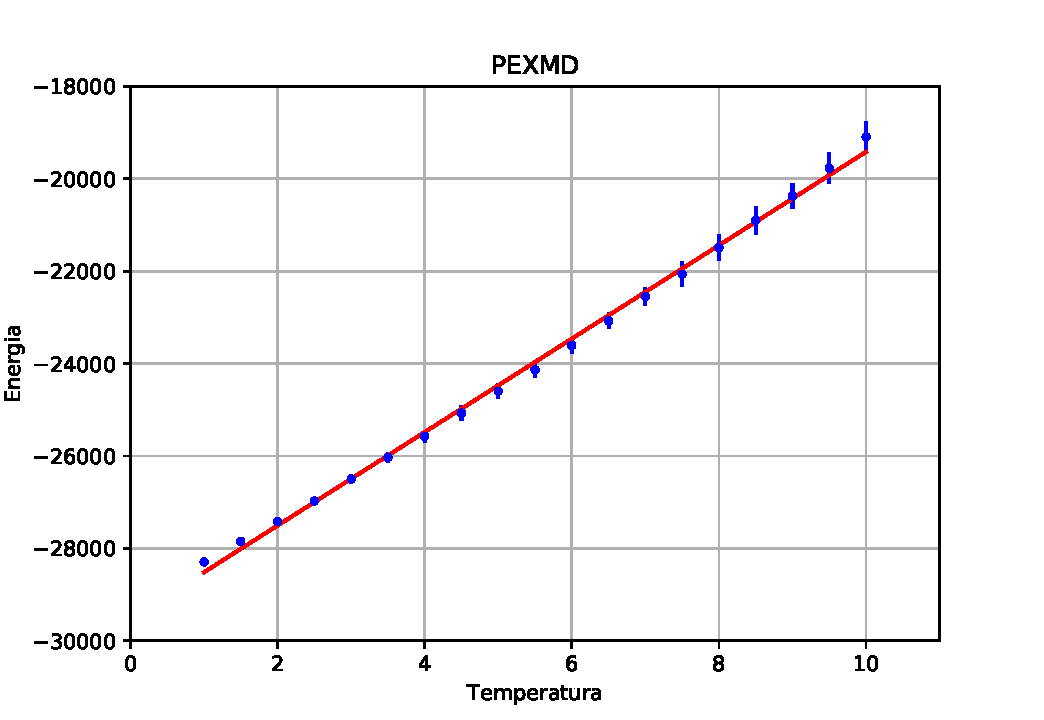
\includegraphics[width=0.48\columnwidth]{evt_pexmd.pdf}
	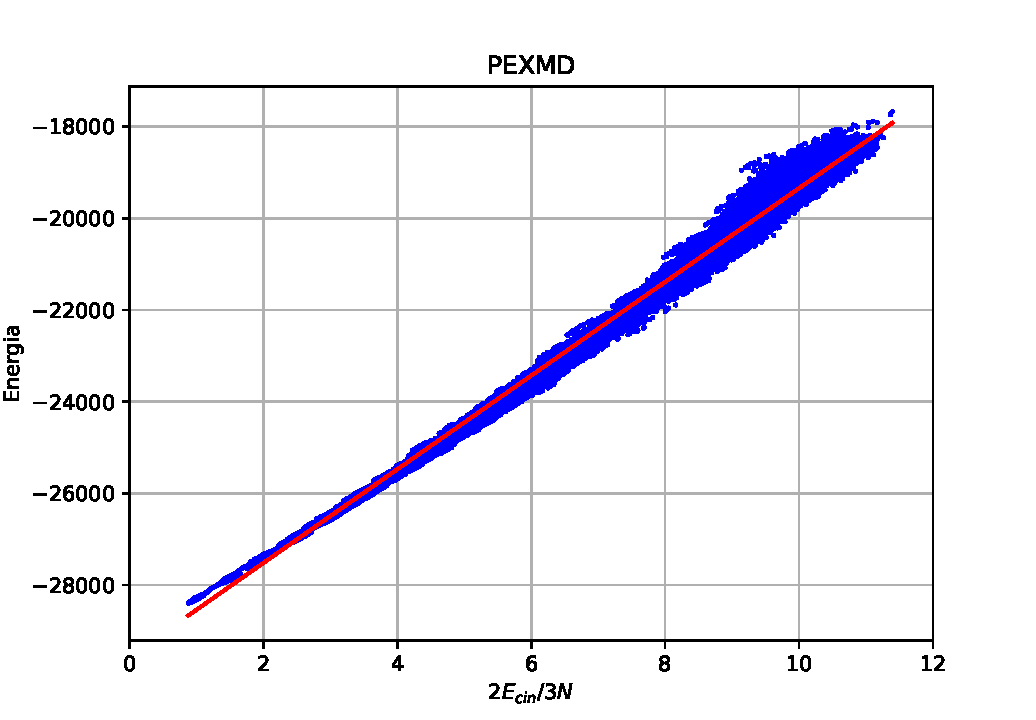
\includegraphics[width=0.48\columnwidth]{evecin_pexmd.pdf}
	\caption{Curvas de Energia vs Temperatura para $T$ (izquierda) y $T_m$ (derecha). Los ajustes arrojan pendientes $m_{pexmd,1}=1011$ y $m_{pexmd,2}=1021$, respectivamente, muy similares 
	a $m_{lammps}=1033$}
	\label{fig:EcinvsT}
\end{figure}


% PEXMD (usando Ecin) m = 1021
% PEXMD (usando termostato) m = 1011

\section{Conclusiones}

En definitiva, pudimos confirmar que la implementación del potencial de Morse en \texttt{PEXMD} es correcta al comparar sus resultados con el de un software reconocido (\texttt{LAMMPS}).
Además, la conservación de la energía es consistente con la implementación NVE de velocity-Verlet.

Más interesantes son las observaciones sobre el comportamiento del potencial de Morse con sus problemas de termalización por reescalamiento de velocidades. 
Practicamente podemos afirmar que este método no es adecuado para este potencial. Sin embargo, la introducción del termostato de Andersen fue exitosa y solucionó este problema.
Su calidad quedó demostrada al punto de poder afirmar que es equivalente usar $T$ y $T_m = 2E_{cin}/3N_{part}$, con fluctuaciones del $3.5\%$. 
Probablemente un $Q\approx0.01$ también tendría estas características, excepto que quizás requeriría una mayor cantidad de pasos de termalización. 

\end{document}